%!TEX root = ../main.tex

\chapter{Fonti energetice}
\label{chp:FontiEnergetiche}
Parlando di fonti energetiche si fa una prima suddivisione di esse in fonti rinnovabili e non rinnovabili, per ciascuna verranno elencati e vari tipo di impianti usati per sfruttarla e trasformarla in energia.

\section{Fonti rinnovabili}
Sono considerate fonti rinnovabili tutte quelle provenienti da:
\begin{itemize}
    \item Irraggiamento solare
    \item Vento
    \item Biomasse
    \item Maree
    \item Correnti marine
    \item Precipitazioni
\end{itemize}
\subsection{Irraggiamento solare}

La radiazione solare è l'energia emessa dal sole, generata a partire da reazioni termonucleari di fusione che avvengono nel sole producendo radiazioni elettromagnetiche a diversa frequenza e lunghezza d'onda le quali trasportano l'energia solare.\\
La radiazione solare che raggiunge il livello più alto dell'atmosfera terrestre è mediamente \(1367\frac{W}{m^2}\) chiamata costante solare (\textit{S}).\\
\textit{S} rappresenta la quantità di energia trasmessa ad un disco di diametro uguale a quello terrestre posto tangenzialmente al livello più alto dell'atmosfera.
%Essendo però la terra assimilabile ad una sfera che ruota attorno al proprio asse,per ottenere il valore medio per unità di tempo di radiazioni che arriva su di essa bisogna quindi considerarne la superficie esterna arrivando ad un valore medio di circa 342$\frac{W}{m^2}$\footnote{Valore considerato sempre nel livello superiore dell'atmosfera}.\\
\newpage\noindent
In buona approssimazione considerando\cite{captazione-enegia-solare}:
\begin{itemize}
    \item fenomeni di riflessione dati dalle nuvole
    \item fenomeni di riflessione dati dalle polveri presenti in atmosfera
    \item fenomeni di interazione chimica con i gas presenti in atmosfera
    \item fenomeni di scattering
\end{itemize}
A causa dei fenomeni elencati sopra,le radiazioni solari che arrivano al suolo presentano quindi due componenti:
\begin{itemize}
    \item diretta, cioè la componente che raggiunge il suolo senza venir in alcun modo perturbata e quindi con la stessa direzione del sole
    \item diffusa, costituita dalla componente che raggiunge il suolo dopo essere stata dispersa,assorbita ed eventualmente re-irraggiata
\end{itemize}
La presenza di due componenti risulta di fondamentale importanza durante il processo di captazione e quindi va tenuta in considerazione durante la scelta della tipologia di impianto da installare, argomento che verrà trattato nel capitolo successivo.
L'industria statunitense in collaborazione con l'ASTM\footnote{American Society for Testing and Materials} ha definito tre standard:
\begin{enumerate}
    \item AM0
    \item AM1.5-f
    \item AM1-37$^\circ$
\end{enumerate}
Prima di andare a spiegare questi tre standard è importante definire un valore m tale da rispettare la seguente proporzione matematica $m=\frac{1}{\cos z}$ come si evince nella figura sottostante:
\begin{figure}[H]
    \centering
    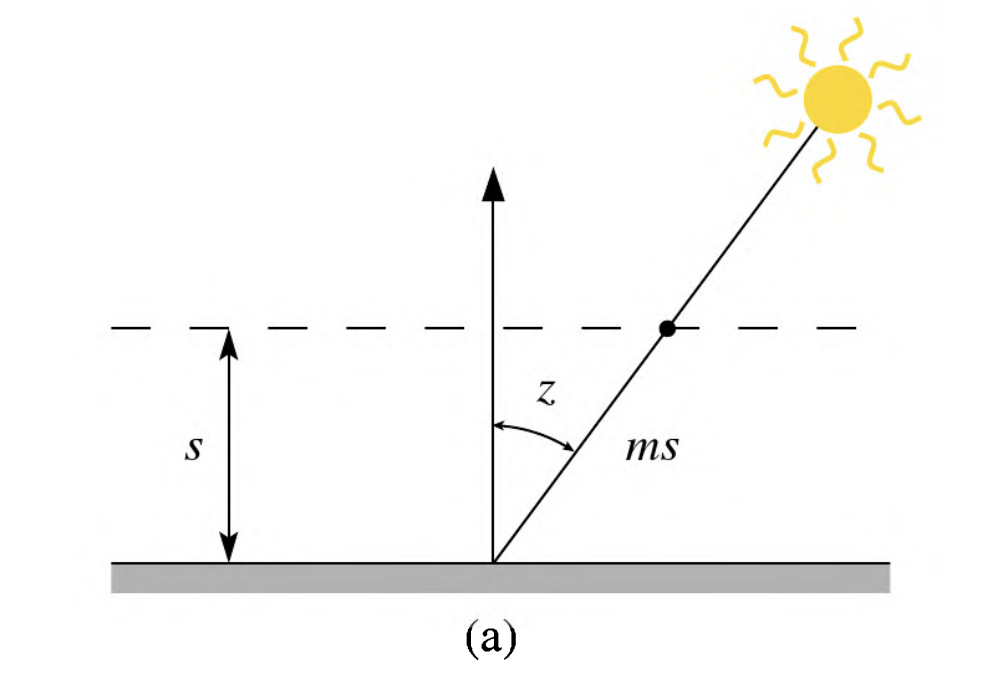
\includegraphics[width=0.4\textwidth]{res/cap2/rappresentazione m}
    \caption{Percorso delle radiazioni solari}
\end{figure}
Il primo standard fa riferimento all'irradianza nel livello più alto dell'atmosfera,
gli altri invece all'irradianza che giunge al suolo dopo un percorso di lunghezza m = 1,5 in un'atmosfera limpida, dove per limpida si considera una visibilità di 23 km.
La seconda fa nello specifico riferimento ad una superficie $A_n$ ortogonale ai raggi solari,la seconda fa riferimento ad una superficie $A_i$ rivolta a sud ed inclinata di un'angolo $\beta = 37^\circ$ rispetto al piano orizzontale, nell'impotesi di un coefficiente di riflessione $\rho_s = 0,2$.
\begin{figure}[H]
    \centering
    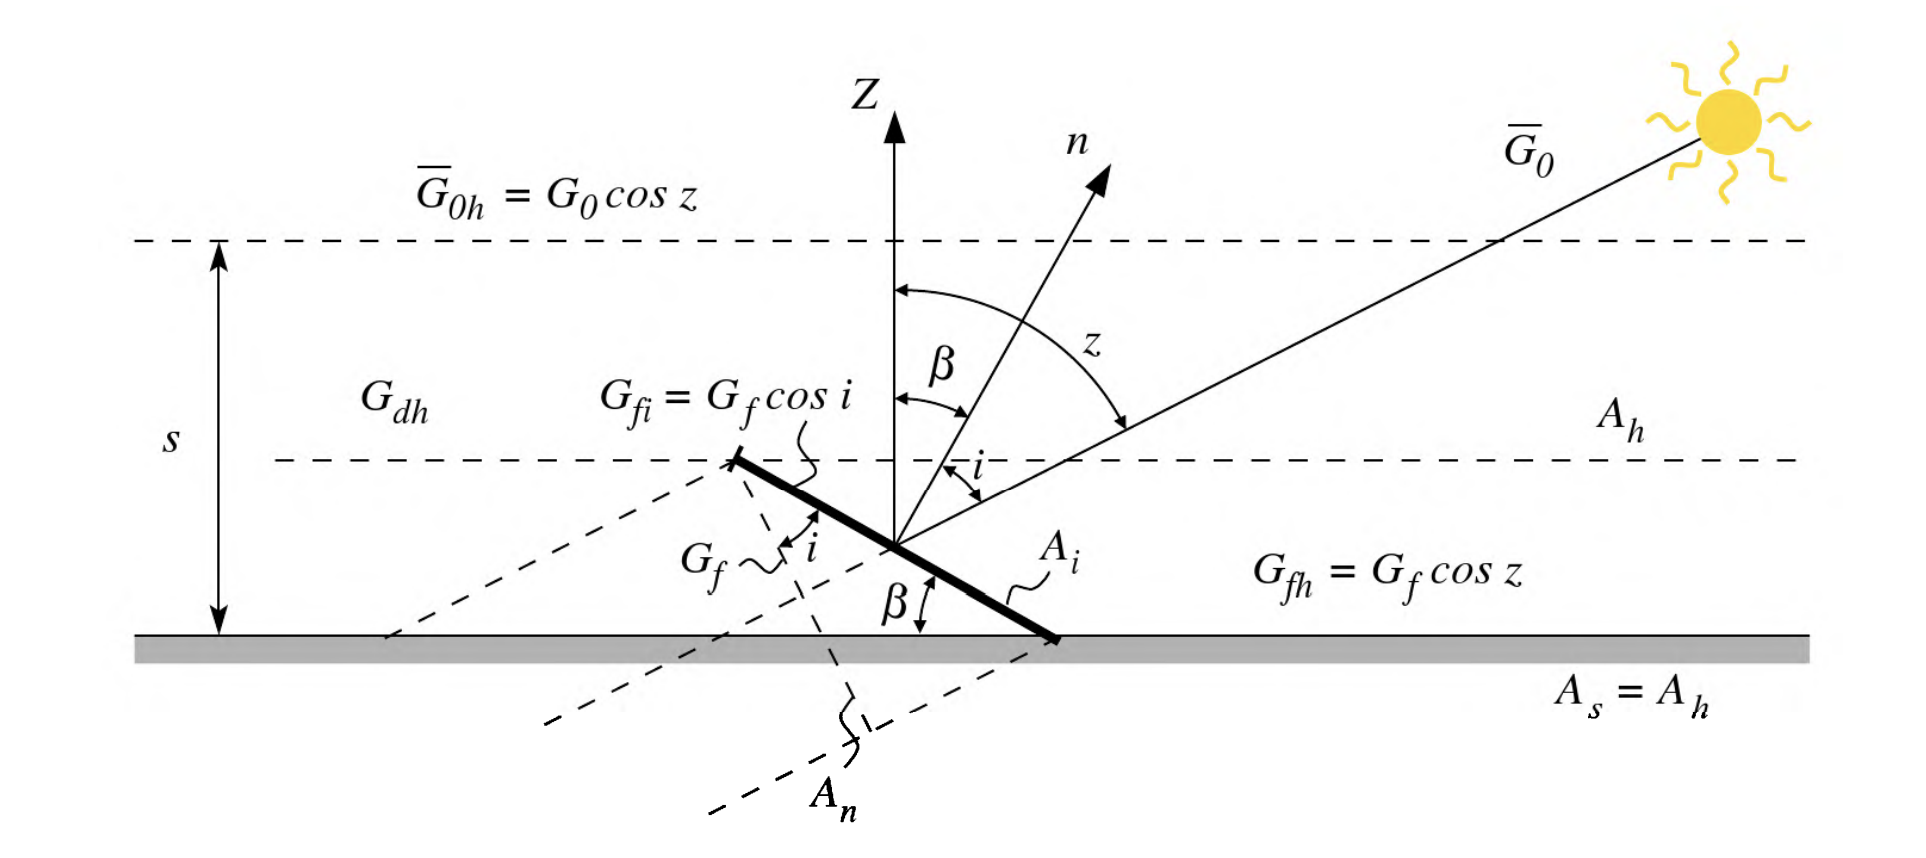
\includegraphics[width=0.8\textwidth]{res/cap2/standard}
    \caption{Rappresentazione superfici stanadard AM1.5-f AM1-37$^\circ$}
\end{figure}
L'energia trasportata dalle radiazioni solari possiamo dividerla sostanzialmente in due componenti:
\begin{itemize}
    \item \textbf{Componente visibile:} quella con lunghezza d'onda [\textbf{$\lambda$}] tra i 400 ed i 700 nm
    \item \textbf{Componenti ad energia minoritaria:} 
        \begin{itemize}
            \item \textbf{ultravioletti} \textbf{$\lambda$} tra i 100 ed i 400nm
            \item \textbf{infrarossi} \textbf{$\lambda$} tra i 700nm ed 1mm
        \end{itemize}
\end{itemize}
Successivamente questa ulteriore suddivisione ci sarà utile per spiegare alcune tecnologie che in grado di lavorare sulle singole componenti.
\begin{figure}[H]
    \centering
    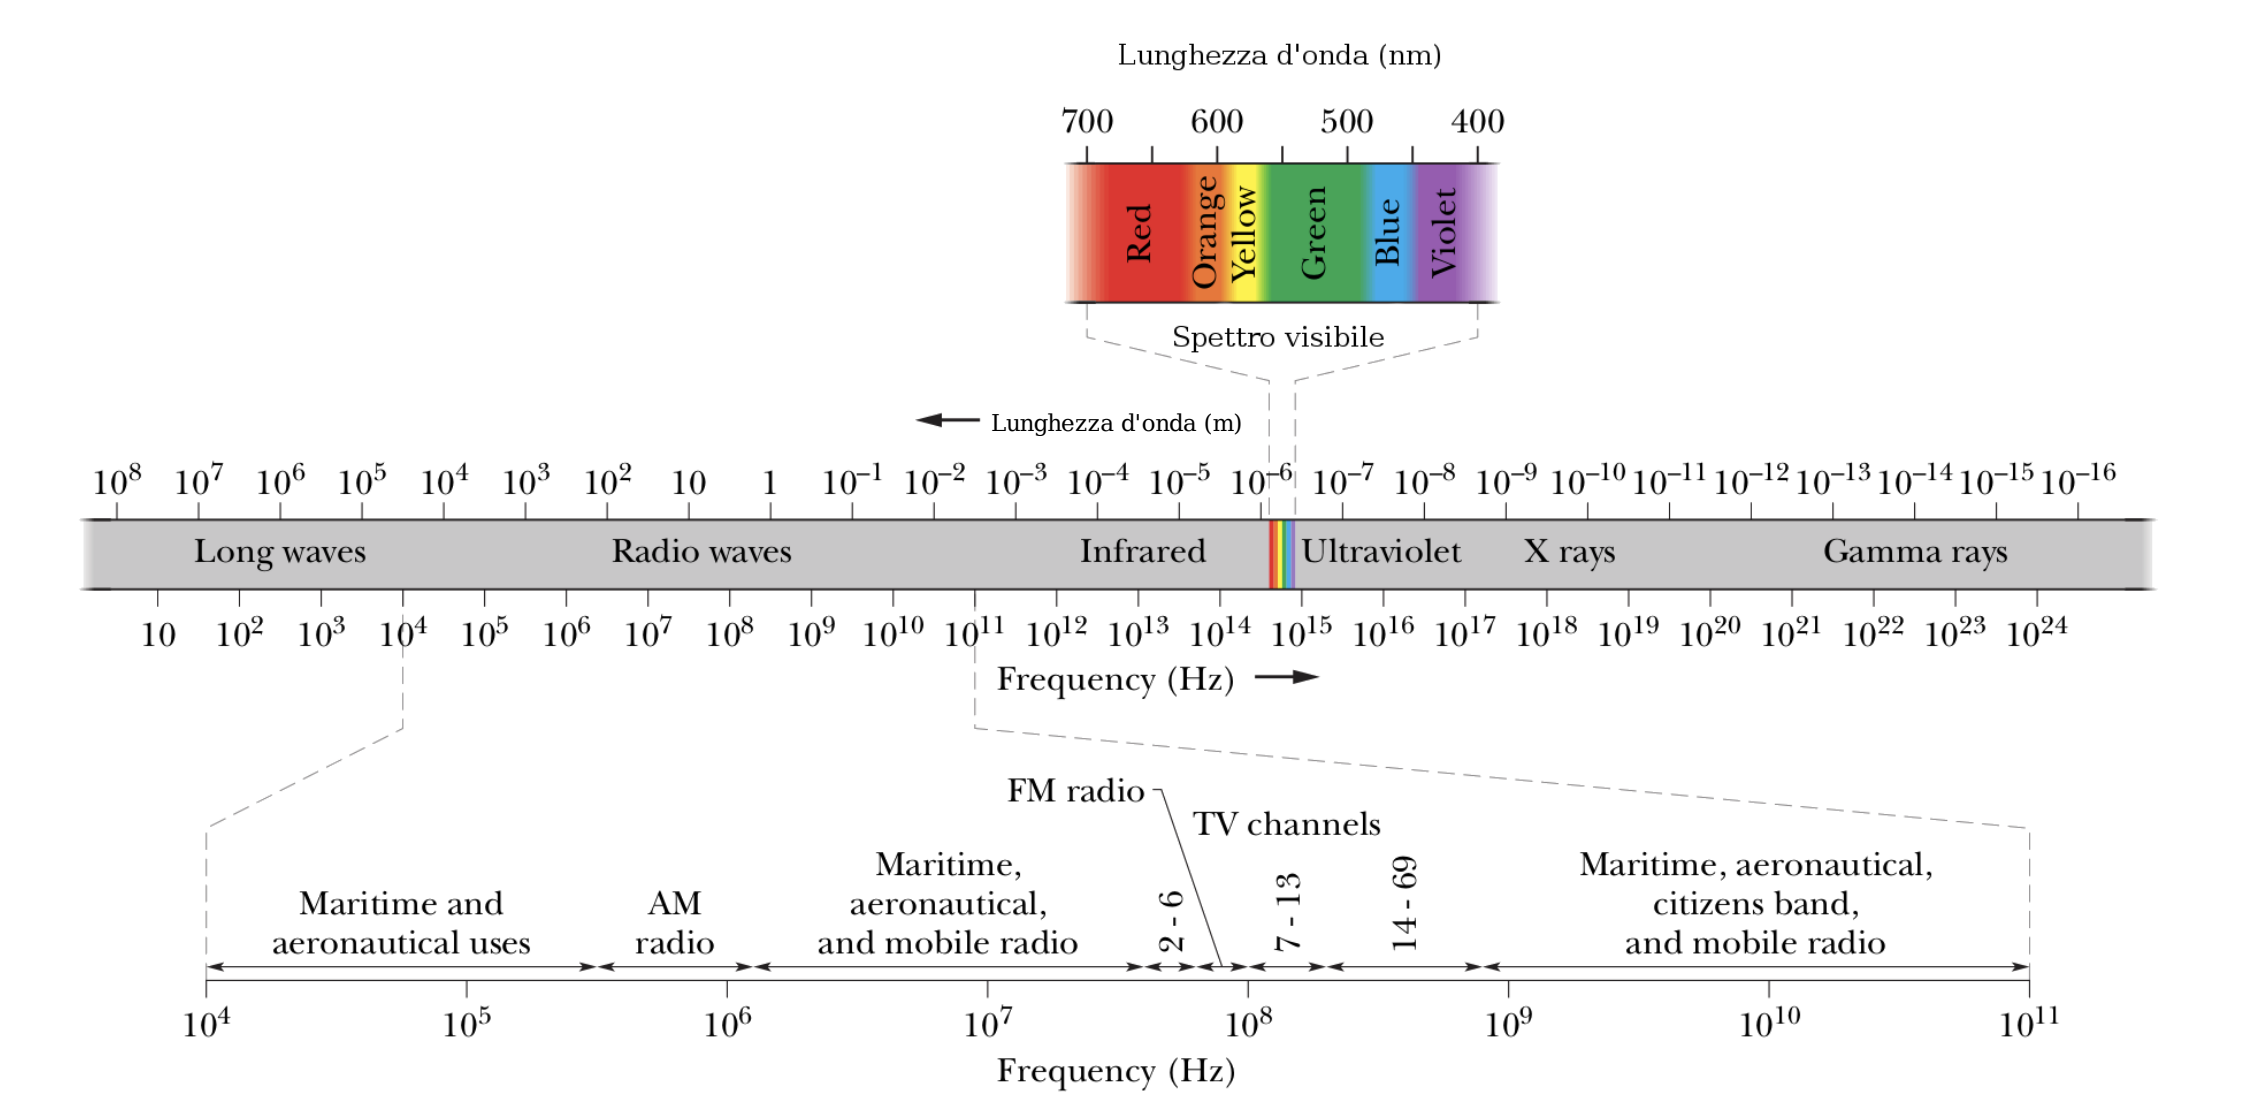
\includegraphics[width=0.8\textwidth]{res/cap2/luce_dettagli}
    \caption{Radiazione solare}
\end{figure}

\newpage
\subsection{Vento}

Quello che comunemente viene chiamato vento è il movimento di una massa d'aria da una regione ad alta pressione ad una a bassa pressione.\\
Quando si parla di vento ci sono diversi aspetti da considerare quali:
\begin{itemize}
    \item Velocità
    \item Densità della massa d'aria
    \item Contenuto energetico
\end{itemize}
\noindent 
Per contenuto energetico si intente l'energia cinetica che l'aria ha in movimento:
\begin{center}
    \large{\(E=\frac{1}{2}\cdot m\cdot v^2 = \frac{1}{2} \cdot(Avt\rho)\cdot v^2 = \frac{1}{2} \cdot(Avt\rho)\cdot v^2 \)}
\end{center}
\noindent
Possiamo notare come l'energia cinetica che la massa d'aria considerata possiede dipende da da tutti i parametri sopra elencati, capire il modo in cui essi partecipano al bilancio energetico ci permetterà nei capitoli successivi di comprendere il funzionamento degli impianti eolici.

\subsection{Biomasse}
Per biomasse intendiamo tutta quella serie di prodotti organici usati per produrre calore od elettricità in specifici impianti appositamente progettate.\\
Sono classificabili in base al fatto che vengano o meno prodotte per generare energia elettrica\cite{IRENA}:
\begin{itemize}
    \item Biomasse primarie
    \item Biomasse secondarie
\end{itemize}
\noindent
Nella prima categoria inseriamo tutto il materiale organico prodotto con lo specifico scopo energetico mentre nella seconda vengono inserite tutti i prodotti organici che sono il risultato di scarti residenziali ed industriali.

\vspace{2mm}
Una volta specificato tutto ciò che è considerabile biomassa andiamo ad elencare le tecniche utilizzate per sfruttare l'energia potenziale contenuta in esse\cite{EIA2022}:
\begin{description}[labelindent=5mm]
    \item[$\bullet$ Conversione termica] in questa tipologia si procede tramite un riscaldamento della biomassa per produrre combustibili in vario stato. In questa categoria sono a loro volta inserite tre tecniche che vanno a loro volta a generate combustibili in diverso stato:
    \begin{description}[labelindent=5mm]
        \item[$\cdot$ Torrefazione:] processo che prevede il riscaldamento della biomassa ad una temperatura compresa tra i 200 ed i 300\degree C in un ambiente quasi privo di ossigeno, dalla biomassa vengono rimosse le componenti a contenuto energetico più basso. Il 30\% viene quindi convertito in gas mentre la restante parte rimane sotto forma di bricchetti solidi o pellet mantenendo però circa l'85\% dell'energia originaria della biomassa\cite{Torrification}. 
        \item[$\cdot$ Pirolisi:] processo che comporta un riscaldamento dei materiali organici ad una temperatura tra i 400 ed i 500\degree C in quasi assenza di ossigeno. Da questo processo vengono generate sostanze quali: bio-oli, carbone, metano ed idrogeno.\\
        Partendo dal bio-olio e tramite un successivo processo di idrotrattamento a temperatura e pressione elevata si possono produrre biocarburanti\cite{EIA2021}.
        \item[$\cdot$ Gassificazione:] processo anch'esso che prevede un riscaldamento delle biomasse ad una temperatura compresa tra gli 800 ed i 900\degree C questa volta però inserendo in modo controllato ossigeno e/o vapore acqueo con l'obbiettivo di produrre \enquote{syngas} il quale potrà poi essere usato per scopi energetici.\cite{EIA2022}
    \end{description}
    \item[$\bullet$ Conversione chimica] questa categoria comprende una serie di processi chimici che hanno lo scopo di trasformare le biomasse in una forma più facile da trasportare ed immagazzinare.\\
    Molti di essi sono simili al processo per produrre \enquote{syngas} spiegato nel punto precedente, un'esempio è un processo chiamato \enquote{transesterificazione} nel quale una sostanza organica viene fatta reagire con dell'alcool per produrre biocarburanti.\cite{EIA2022}
    \item[$\bullet$ Conversione biologica] in questa sezione sono inseriti tutti quei processi che sfruttano microrganismi per un processo di conversione, tra questi cito: digestione anaerobica, fermentazione e compostaggio.\\ Lo scopo è quello di trasformare la biomassa in sostanze quali bioetanolo o biogas. 
\end{description}

\subsection{Maree}
Le maree sono il naturale cambiamento del livello del mare causato da una combinazione di effetti gravitazionali della luna, del sole e legati alla rotazione terrestre.\\Il cambiamento di marea attraversa due stati fondamentali,quando il livello smette di diminuire raggiungendo un minimo locale ci troviamo in uno stato chiamato bassa marea, viceversa quando smette di crescere raggiunge uno stato di massimo locale parliamo di alta marea.\\
Sono presenti,in prima approssimazione, due componenti fondamentali le quali poi avranno anch'esse delle componenti specifiche chiamati costituenti:\\

\vspace{0,5em}\noindent
\begin{tabular}{|c|c|c|c|}
\hline
\multicolumn{4}{|l|}{Semi-diurna}\\
\hline
Costituente & Periodo(h) & Velocità($\degree$/h) & Ampiezza(cm) \\ 
\hline
M2  & 12.421 & 28.984 & 58  \\ \hline
S2  & 12 & 30 & 13.7  \\ \hline
N2  & 12.658 & 28.439 & 12.3  \\\hline
\end{tabular}\\

\vspace{1em}\noindent
\begin{tabular}{|c|c|c|c|}
\hline
\multicolumn{4}{|l|}{Diurna}\\
\hline
Costituente & Periodo(h) & Velocità($\degree$/h) & Ampiezza(cm) \\ 
\hline
K1  & 23.934 & 15.041 & 36.8 \\ \hline
O1  & 25.819 & 13.943 & 23.0 \\ \hline
P1 & 24.066 & 14.958 & 11.6 \\\hline
\end{tabular}\\

\vspace{1em}
\noindent
I dati riportati nelle tabelle soprastanti ci indicano le componenti principali riferite ad una determinata posizione geografica presa come esempio, sono state riportate solamente le principali in quanto tramite esse è possibile ottenere una buona approssimazione sull'andamento della marea\footnote{Dati ricavati dal sito del National Oceanic and Atmospheric Administration della città di San Francisco}.

\begin{figure}[H]
    \centering
    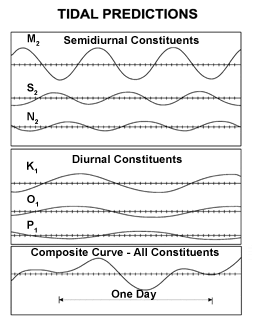
\includegraphics[width=0.3\textwidth]{res/cap2/Tidal_constituent_sum}
    \caption{Curva ottenuta dai costituenti}
\end{figure}

Si nota come la curva ottenuta sia la somma delle componenti, essa rappresenta l'andamento della marea dato dalle componenti principali e più rilevanti.\\
Ci sono inoltre fattori influenzano l'andamento delle maree che non dipendono solamente dai puri dati numerici sopra indicati correlati all'orario od alla stagione in cui ci si trova ma anche dalla realtà in cui ci si trova geografica si trova.\\
Il livello del mare nelle coste francesi mediterranee ad esempio oscilla meno di quanto avviene sulle coste francesi che danno sull'oceano in quanto la presenza di stretti non permette all'acqua di mantenere un'andamento di discesa/salita lineare ma lo altera. Da qui la difficoltà maggiore di riuscire a creare un modello predittivo affidabile per realtà particolare quali la città di Venezia a esempio.
\newpage
\subsection{Correnti marine}
Con corrente marina intendiamo una massa d'acqua in movimento rispetto a quella che la circonda e che può avere una differente densità,salinità o temperatura.\\
Gli effetti principali che provocano la formazione di queste correnti sono:\cite{NOAA-current}
\begin{itemize}
    \item Effetto di Coriolis
    \item Differenza di temperatura
    \item Differenza di salinità
    \item Rottura del moto ondoso
    \item \enquote{Cabbeling}
\end{itemize}\noindent
Si parla di \enquote{Cabbeling} quando abbiamo due basse d'acqua denominate con A e B le quali andando a mescolarsi formeranno una nuova massa d'acqua che ha una densità superiore a quella di A e B
\begin{figure}[H]
    \centering
    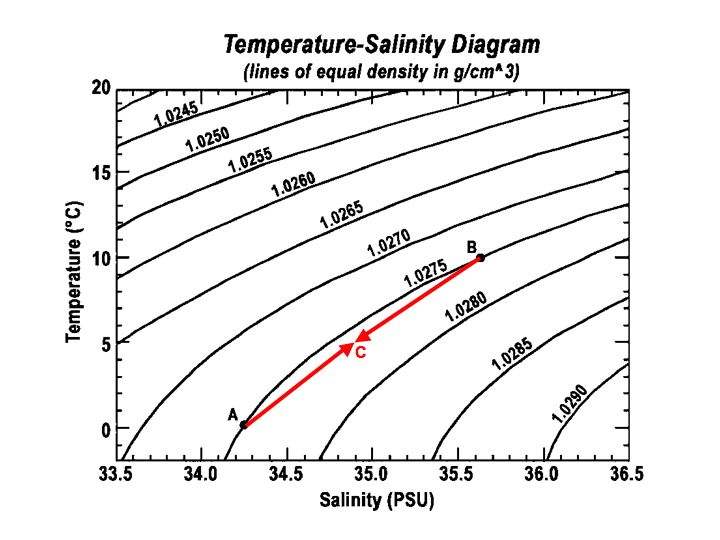
\includegraphics[width=0.5\textwidth]{res/cap2/temperature-salinity}
    \caption{Diagramma Temperatura salinità ed effetto "Cabbeling"}
\end{figure}\noindent
La dinamica che descrive le varie correnti parte da una divisione dell'oceano in tre livelli:
\begin{itemize}
    \item \textbf{Strato misto:} è uno stato superficiale le cui proprietà fisiche variano nel tempo e le cui correnti sono generate dagli strati inferiori
    \item \textbf{Oceano superiore:} sopra la linea termoclina
    \item \textbf{Oceano profondo:}  sotto la linea termoclina
\end{itemize}\noindent
Con linea termoclina identifichiamo un livello nella quale avviene un'importante rimescolamento dell'acqua e nel quale c'è quindi una più veloce variazione di temperatura, un'esempio si può vedere nel grafico riportato sotto:
\begin{figure}[H]
    \centering
    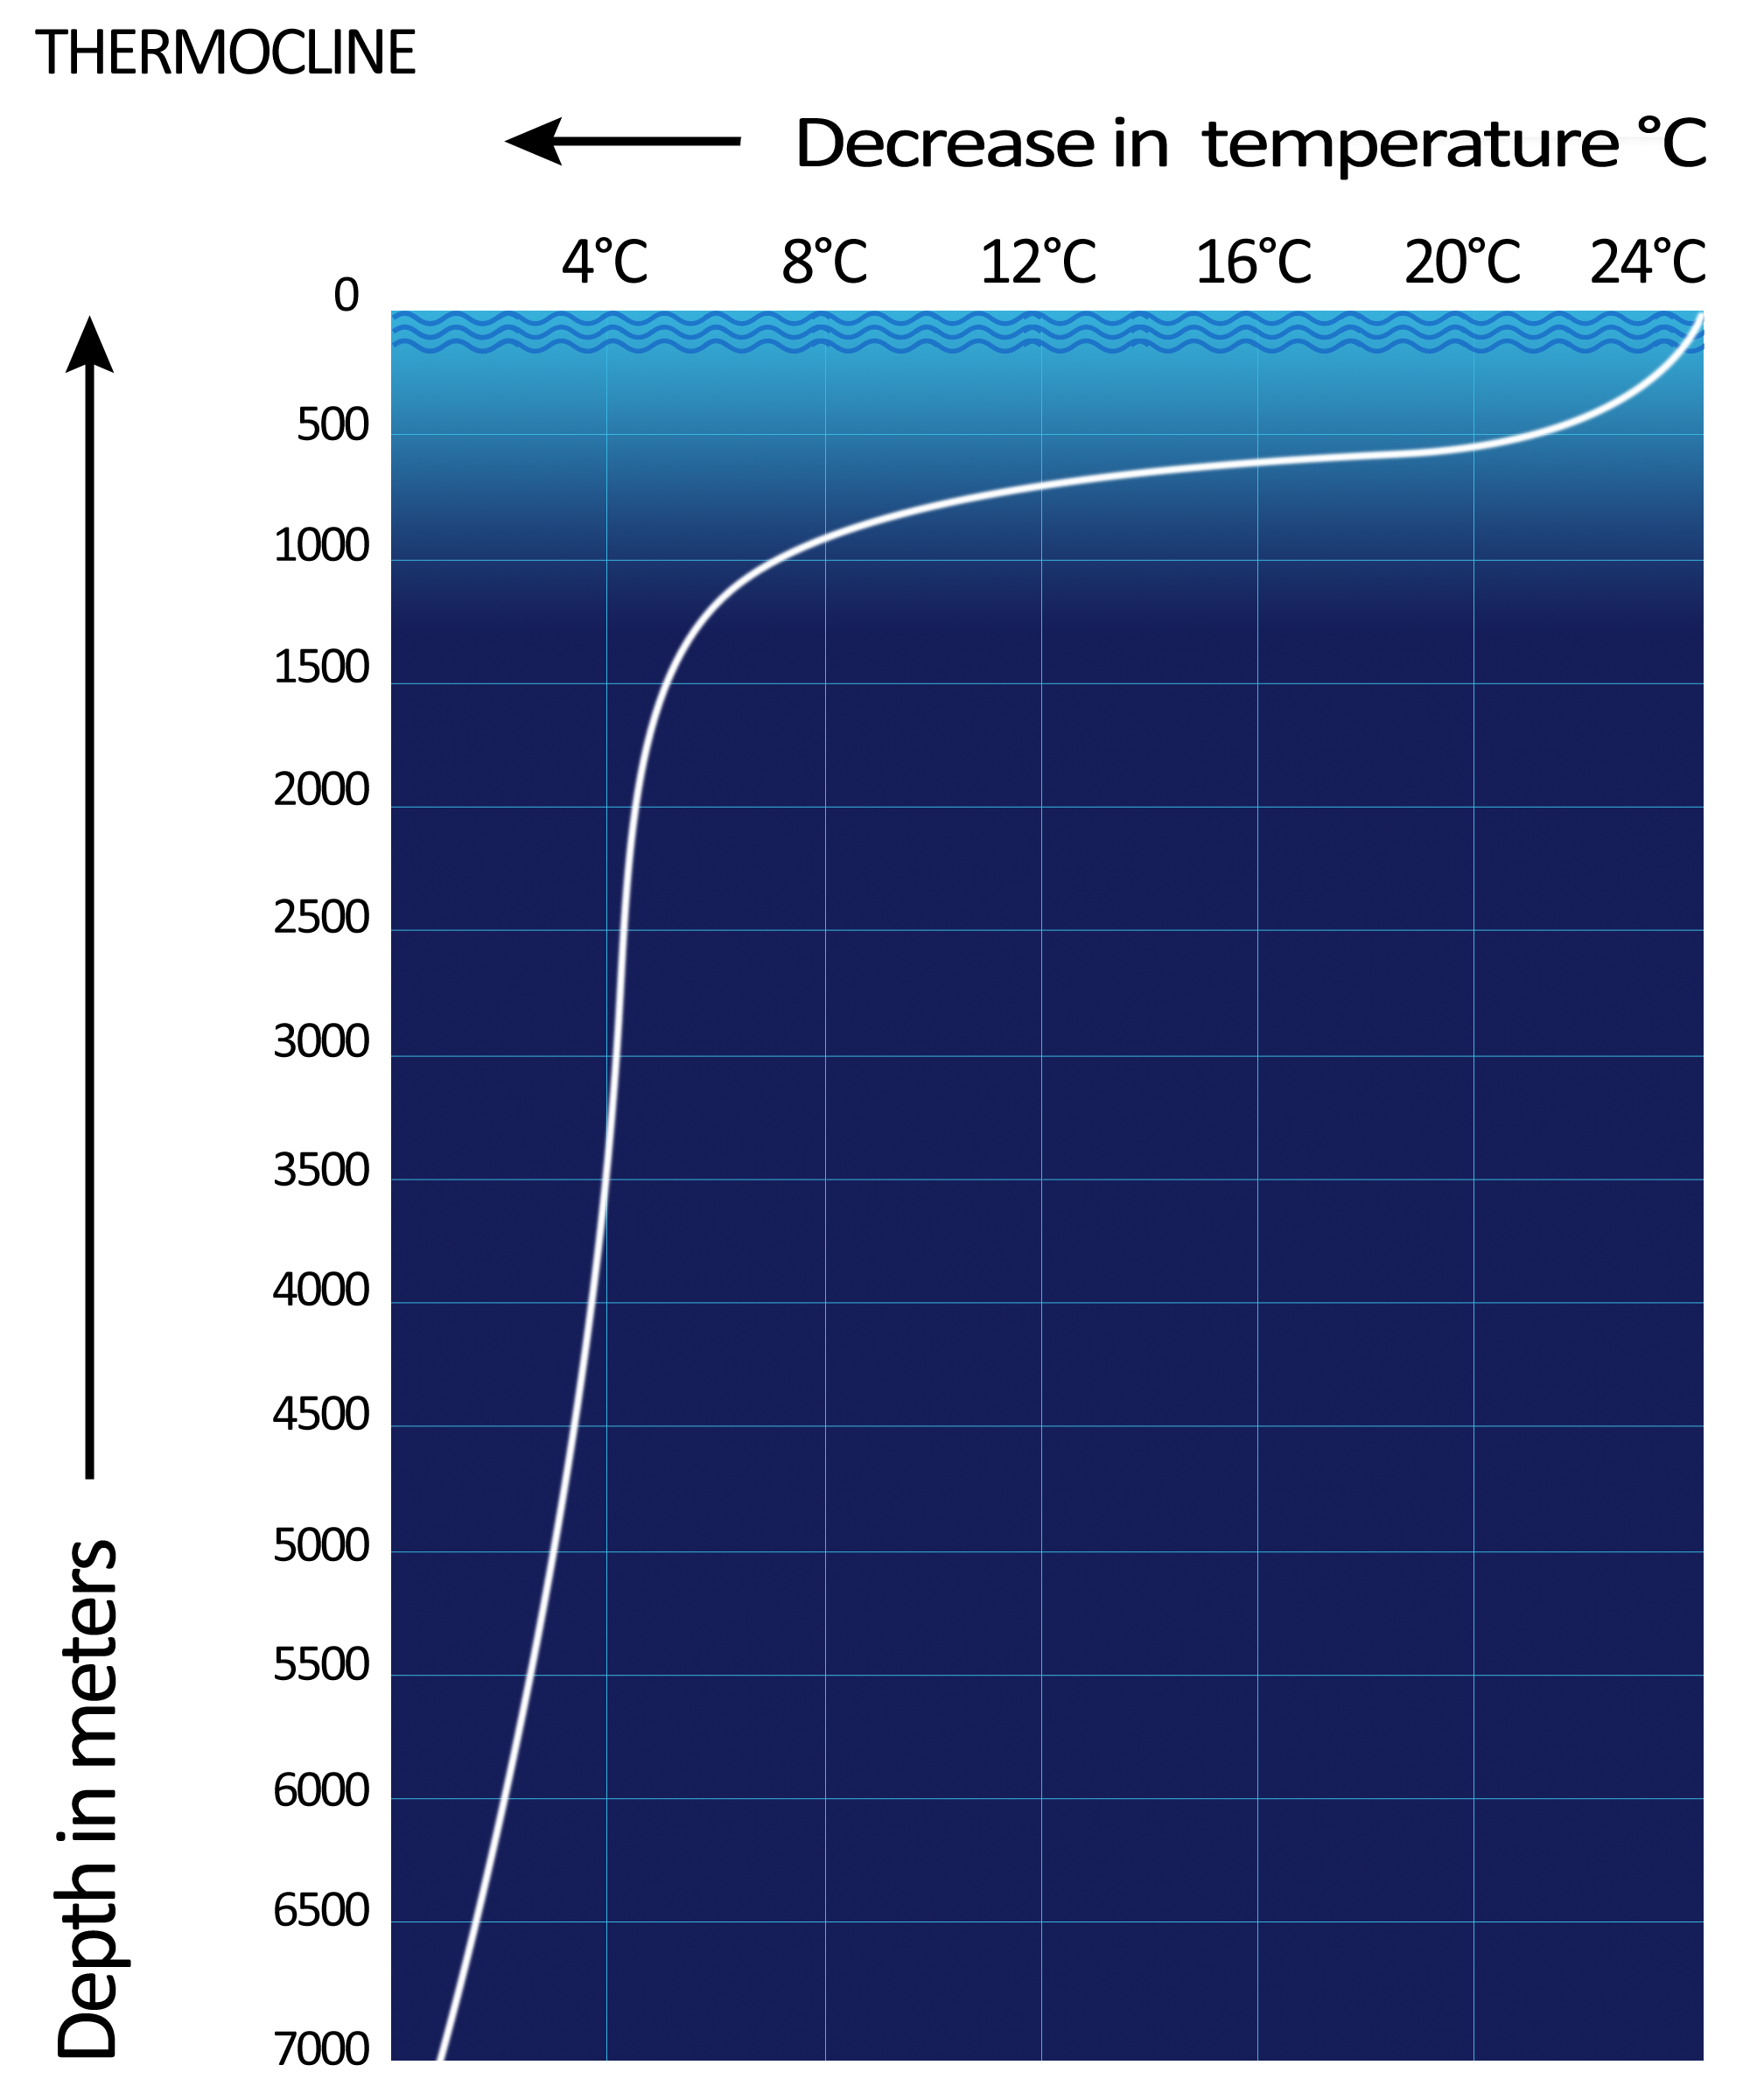
\includegraphics[height=0.4\textwidth]{res/cap2/termoclino}
    \caption{Variazione di temperatura in funzione della profondità}
\end{figure}\noindent
Tutte le corrente oceaniche di superficie sono solitamente guidate da correnti ventose, venti che sono influenzati in gran parte dall'effetto di Coriolis sopra citato.\\
Le correnti più profonde sono mosse da un fenomeno chiamato: \enquote{Circolazione termoalina}.
Esso è a sua volte correlato a fenomeni fisici legati alla variazione di densità e di temperatura, i principali agenti che provocano una variazione di temperatura o densità sono il calore proveniente da livelli superiori e la differenza di densità provocata da grandi flussi d'acqua dolce provenienti sempre da i livelli superiori.\\

\subsection{Precipitazioni}
Le precipitazioni sono un fenomeno atmosferico che porta il vapore acqueo contenuto nell'atmosfera,una volta condensato, a cadere per l'effetto della gravità.\\
L'aria contiene vapore acqueo e la sua quantità varia molto da zona a zona e quindi non è comunemente inserita negli elementi che compongono l'aria.\\
Per esprimerne il quantitativo contenuto in atmosfera si usano diversi metodi:
\begin{itemize}
    \item Rapporto volumetrico: $(\frac{volume\,  d'acqua}{volume\,  d'aria})$
    \item Umidità specifica: rapporto in massa tra quantità di vapore e quantità di aria  $(\frac{g\, H_2O}{kg\, aria})$
    \item Mixing ratio: rapporto tra la quantità di vapore acqueo e quella d'aria secca $(\frac{g\, H_2O}{kg\, aria\, secca})$
    \item Umidità assoluta: densità di vapore acqueo $(\frac{g\, H_2O}{m^3\, aria})$
    \item Umidità relativa: rapporto tra la pressione parziale di acqua e la pressione di saturazione dell'acqua ad una determinata temperatura $(\frac{p_{H_2O} }{p_{H_2O}^s})\%$
\end{itemize}
L'incontro di masse d'aria aventi temperature diverse porterà quella a temperatura maggiore a salire generando una zona a bassa pressione, salendo la temperatura della massa calda e la pressione inizieranno a scendere fino a far incontrare al vapore condizioni che gli permette di condensare e quindi di cadere a terra generando fenomeni di rovesci.\\
\newpage
\section{Fonti non rinnovabili}
Sono considerate non fonti rinnovabili:
\begin{itemize}
    \item Gas naturale
    \item Carbone
    \item Petrolio
    \item Uranio
\end{itemize}
Ad eclusione dell'uranio, per ciascuna verrà fatto un breve excursus sulla formazione, sul potere calorifero che è in grado di offrire anche in relazione al suo prezzo di mercato. Verranno riportati i prezzi presi da un noto sito governativo già citato in precedenza presi tutti nello stesso periodo e opportunamente convertiti in unità per renderli paragonabili.\\
Parlando di prezzi è importante precisare come i prezzi indicati siano puramente indicativi e relativi ad un determinato mercato e non tengano conto di voci di costo importanti quali: gli impianti necessari a trasportarli e la importante differente strutturale e quindi di costo degli impianti di generazione.\\
\subsection{Gas naturale}
Quando si parla di gas naturale si indica una miscela di più gas:
\begin{itemize}
    \item Metano($C H_4$)
    \item Etano ($C_2 H_6$)
    \item Propano ($C_3 H_8$)
    \item Butano ($C_4 H_10$)
    \item Anidride carbonica ($C O_2$)
    \item Azoto ($N_2$)
    \item Ossigeno ($O_2$)
    \item Gas nobili(tracce)
\end{itemize}
Si può subito notare come il gas naturale non contenga solo idrocarburi ma contenga anche altri gas i quali vanno considerati sia durante il bilancio energetico che durante il trattamento degli inquinanti.\\
In prima analisi possiamo immaginare una combustione ideale di metano:
\begin{center}
    \ch{CH4\gas{} + 2 O2\gas{}->CO2\gas{} + 2 H2O\gas}
\end{center}
Per il calcolo dell'energia sprigionata dalla reazione useremo la legge di Hess la quale conoscendo tramite apposite tabelle i $\Delta H$ di formazione dei vari componenti ci permette di conoscere quella dell'intera reazione.
\begin{center}
    \large{$\Delta H_{rz} = \Delta H_{f,CO_2}(T) + 2\Delta H_{f,H_2O}(T) - \Delta H_{f,CH_4}(T) - \Delta H_{f,O_2}(T) $}
\end{center}
Sostituendo i valori ottenuti sperimentalmente e poi tabulati\footnote{https://cccbdb.nist.gov/xp1.asp?prop=1} otteniamo:
\begin{center}
    \large{$\Delta H_{rz} = -803070\frac{Kj}{Kmol} $}
\end{center}
A questo punto possiamo ottenere il potere energetico di un Kg di metano:
\begin{center}
    \large{$\frac{\Delta H_{rz}}{PM_{CH_4}} = \frac{-803070}{16.042} = -50060 \frac{Kj}{Kg} \sim -35.83 \frac{MJ}{Nm^3}$\footnote{Metro cubo normale(1atm e 0\degree C)}}
\end{center}
\newpage\noindent
Parlando di combustibili è importante citare due caratteristiche cioè:
\begin{itemize}
    \item Potere calorifero inferiore(LHV)
    \item Potere calorifero superiore(HHV)
\end{itemize}
\smallskip
\noindent
Il primo non tiene conto del calore latente di vaporizzazione dell'acqua generata durante la combustione mentre il secondo ne tiene conto.\\
E' importante esprimere entrambi i valori in quando nei moderni impianti si è in grado di utilizzare anche il delta energetico tra il limite superiore ed inferiore andando quindi a sfruttare meglio le risorse ed ad aumentare i rendimenti.\\
Quello calcolato in precedenza avendo nella reazione l'acqua in uscita in forma gassosa corrisponde al LHV, per calcolare l'HHV bisogna tenere in considerazione la quantità di energia che va sottratta a al vapore per farlo condensare:
\begin{center}
    \large{$\Delta H = 2 \cdot -44010 = -88020 \frac{Kj}{Kmol} \Rightarrow \frac{-88020}{18.016}[\frac{\Delta H}{PM_{H_2O}}] = -4886 \frac{Kj}{Kg}$}
\end{center}
Sommando il valore ottenuto a quello precedentemente calcolato possiamo trovare l'HHV:
\begin{center}
    \normalsize{$HHV = \Delta H_{rz} + \Delta H_{cond} = -803070 + (-88020) = -891090 \frac{Kj}{Kmol}\sim -55547 \frac{Kj}{Kmol} \sim -39.76 \frac{MJ}{Nm^3}$}
\end{center}
Tutti i segni negativi sono dovuti al fatto che la reazione presa in considerazione sia esoergonica.\\
L'energia liberata che sarà sotto forma di energia termica potrà poi essere opportunamente trasformata o direttamente utilizzata.\\
Il prezzo riportato per il gas naturale in questo caso è in $\frac{\$}{million BTU}$ ed quivale a 6,60\$ che riportandolo in unità del S.I. equivale a $0,0062\frac{\$}{MJ}$.\\
\noindent
\newpage
\subsection{Carbone}
Sono presenti diverse tipologie di carbone, i quali si differenziano inizialmente per fossili e non fossili.\\
Tra i carboni fossili troviamo:
\begin{itemize}
    \item Torba
    \item Lignite
    \item Litantrace
    \item Antracite
\end{itemize}
Si differenziano per una crescente percentuale di carbonio e per la diminuzione progressiva dell'umidità contenuta.\\
Per andare a proporre un bilancio energetico come per il gas naturale è stato anche qui necessario fare delle semplificazioni, il tutto è iniziato con un'analisi su quale fosse il carbone fossile maggiormente utilizzato negli anni per capire quale convenisse prendere in esame:\cite{EIA-Statistics-World}\\
\begin{figure}[H]
    \centering
    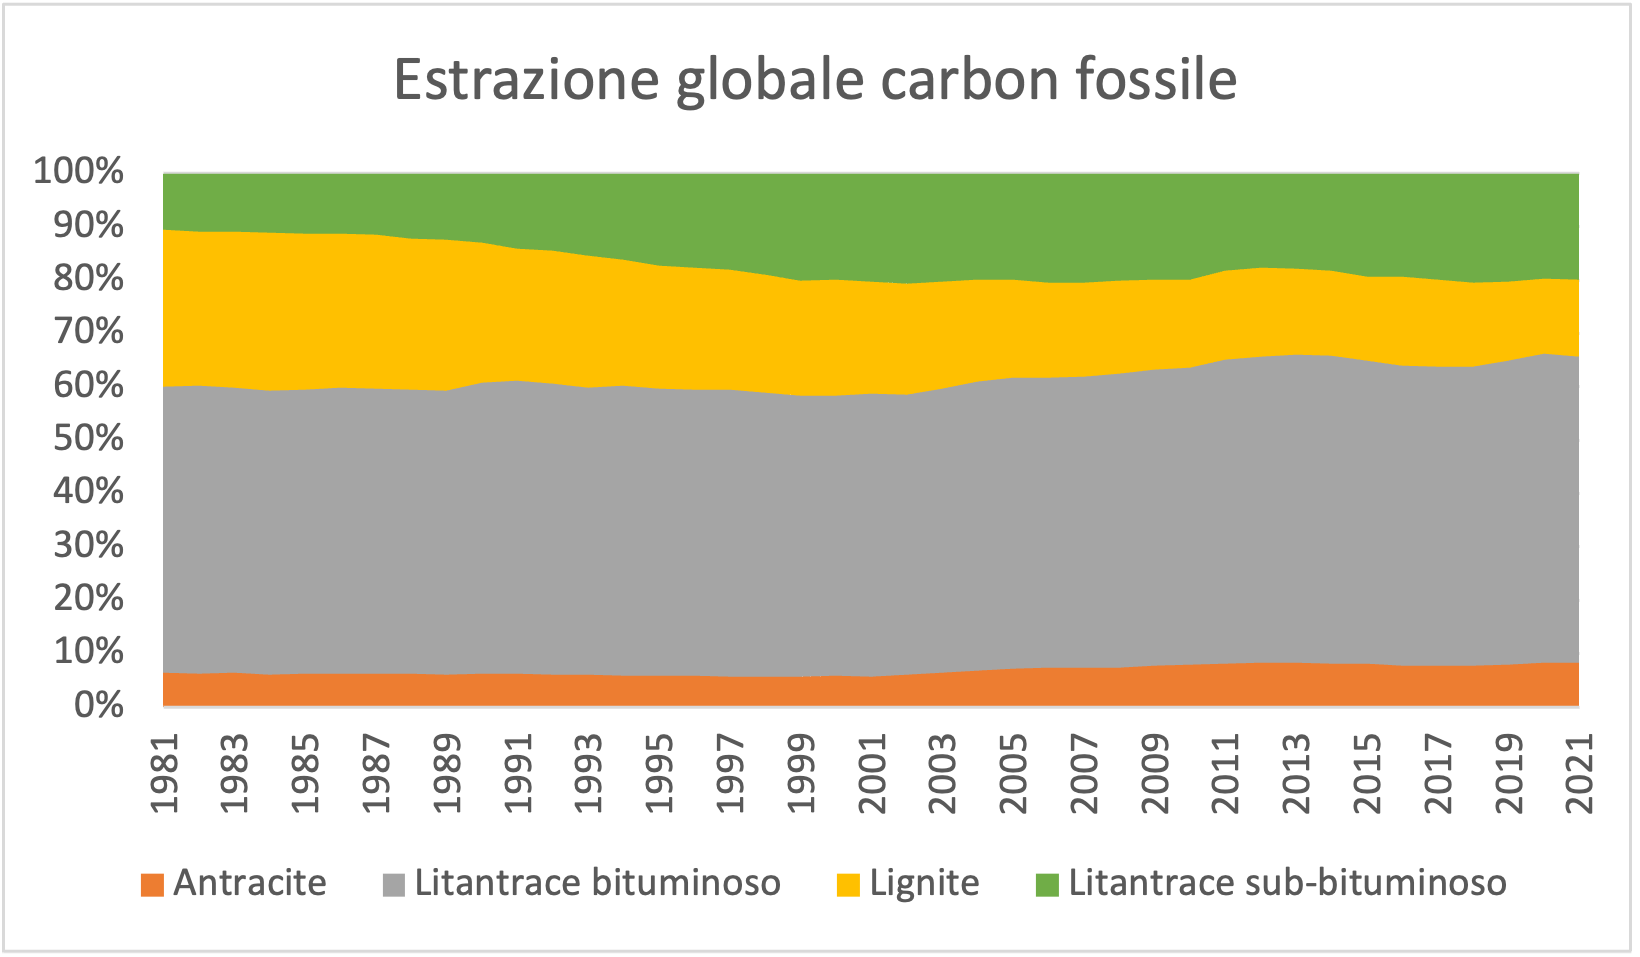
\includegraphics[height=0.6\textwidth]{res/cap2/Grafico carbone}
    \caption{Grafico rappresentate la quantità di carbone estratta globalmente negli ultimi 40 anni}
\end{figure}\noindent
Prenderemo quindi il litantrace bituminoso il quale è il più largamente estratto e consumato, risulta che abbia la seguente composizione in peso:\cite{Composizione-antracite}\\
\begin{itemize}
    \item Carbonio(84.4\%)
    \item Ossigeno(6.7\%)
    \item Idrogeno(5.4\%)
    \item Azoto(1.7\%)
    \item Zolfo(1.8\%)
\end{itemize}
Si noti come in questo caso vi è un contenuto anche di altre sostante oltre ad idrogeno e carbonio tra le quali si evidenzia lo zolfo la cui presenza porta a dei residui di combustione altamente impattanti a livello ambientale.\\
Data la formazione chimica più complessa andare a portare una grossa semplificazione come fatto in precedenza riporterebbe un dato totalmente falsato e poco significativo; per questo motivo sarà riportato il valore contenuto in alcune tabelle che si attesta attorno ai  $20\frac{KJ}{Kg}$ valore che spesso, data la formazione chimica del carbone che può variare di molto da giacimento a giacimento, viene calcolato sperimentalemente.\\
Il prezzo riportato in questo caso è in $\frac{\$}{short ton}$ una \enquote{short ton} equivale a 2000lb quindi a circa 907kg, tenendo conto del potere calorifero riportato in precedenza si arriva ad un valore finale di circa $0,01\frac{\$}{MJ}$.
\subsection{Petrolio}
Il petrolio una volta estratto deve subire diverse lavorazioni prima di poter venir usato per produrre energia, il processo che porta il petrolio ad essere frazionato è quello della distillazione.\\
Il processo di lavorazione del petrolio si compone di diverse fasi le quali avvengono in sequenza sui diversi componenti estratti per andare a sfruttare al massimo la materia prima.\\
La componente che per questa sezione ci interessa è quella degli oli combustibili i quali sono oli pesanti utilizzati prevalentemente per la produzione di energia in centrali termoelettriche e per il settore navale sempre come combustibile.
Anche in questo caso il problema dell'utilizzo di queste sostanze come combustibile è l'alto tenore di zolfo che contengono il quale una volta avvenuta la combustione andrà a combinarsi con l'ossigeno e l'idrogeno contenuti in atmosfera andando a generare acido solforico e acido nitrico provocando i fenomeni comunemente chiamati piogge acide.\\
Da un barile di petrolio\footnote{42 galloni statunitensi $\sim$159 litri} si ricavano circa 45 galloni di prodotti raffinanti con la suddivisione indicata nella tabella sottostante\cite{composizione-petrolio}:\\
\begin{table}[!ht]
    \centering
    \begin{tabular}{|l|l|l|}
    \hline
        \textbf{Prodotto} & \textbf{Quantità[gal]} & \textbf{\%} \\ \hline
        Finished motor gasoline & 20,08 & 45,07\% \\ \hline
        Distillate fuel oil & 12,47 & 27,99\% \\ \hline
        Kerosene-type jet fuel & 3,53 & 7,92\% \\ \hline
        Petroleum coke & 2,06 & 4,62\% \\ \hline
        Still gas & 1,72 & 3,86\% \\ \hline
        Hydrocarbon gas liquids & 1,68 & 3,77\% \\ \hline
        Asphalt and road oil & 0,92 & 2,07\% \\ \hline
        Residual fuel oil & 0,59 & 1,32\% \\ \hline
        Naptha for feedstocks & 0,46 & 1,03\% \\ \hline
        Lubricants & 0,46 & 1,03\% \\ \hline
        Other oils for feedstocks & 0,25 & 0,56\% \\ \hline
        Miscellaneous products & 0,21 & 0,47\% \\ \hline
        Special napthas & 0,08 & 0,18\% \\ \hline
        Finished aviation gasoline & 0,04 & 0,09\% \\ \hline
        \textbf{TOTALE} & \textbf{44,55} & \\ \hline
    \end{tabular}
\end{table}\\
Per ogni barile di petrolio grezzo dopo la raffinazione rimangono quindi 0,59 galloni di olio combustibile che è il prodotto che ci interessa per questa sezione.
Facendo riferimento anche in questo caso a dati tabulati troviamo che il potere calorifico dell'olio combustibile è di $41,022 \frac{MJ}{kg}/$, dopo le opportune conversioni otteniamo un valore di $0,00017\frac{\$}{MJ}$.
Non sono neanche in questo caso stati inseriti i costi di estrazione, trasporto e successiva raffinazione.